% !TeX root = ../main.tex

\chapter{强相互作用玻色超流体中的拓扑Higgs模}
\label{ch3}

\section{背景介绍}

在上一章,我们讨论了弱相互作用玻色超流体Bogoliubov谱中对称性保护的拓扑能带。从直观来说,其能带拓扑的存在性是容易理解的:弱相互作用极限下的Bogoliubov激发谱在高能区域和无相互作用能带几乎没有区别,所以在高能处带隙间的拓扑边界态不会消失。尽管如此,上章的重点是考察有赝时间反演对称性保护的能带拓扑,这一点并不显然:事实上正如我们在附录\ref{mfs}里展示的那样,当相互作用形式改变时,即使总哈密顿量存在通常意义上的时间反演对称性,有效哈密顿量的赝时间反演对称性也可能消失。另外需要注意,由于伽利略不变性,低能极限下的相位扰动和振幅扰动是共轭变量,这对共轭变量只会给出一支Goldstone模。

我们知道,一个连续对称性的自发对称破缺会导致两类序参量的集体振荡模式:无质量的Goldstone模式和有质量的Higgs模式。在粒子物理里,所谓的Higgs玻色子\cite{Higgs1964}是被一个规范的玻色凝聚体模拟的;通过Higgs机制,它产生了各种基本粒子的质量。在凝聚态物理中类似的例子更丰富:例如电荷密度波\cite{Yusupov2010}, 超导体 \cite{Tsuchiya2018}, 量子磁体 \cite{Su2020}, 光晶格中的冷原子凝聚体\cite{Liu2015}等等。在这些体系中,Higgs模是一种集体的复序参量或者向量场振幅的波动。

关于以上两个基本概念,一个很有意思问题是:在强相互作用的量子相变点附近有涌现的拓扑Higgs模?或者反过来问,低能的拓扑激发模在量子相变点附近能不能变成完全的Higgs模式?
这章中,通过研究一个简单的、在冷原子体系中容易实现的模型,我们将对这个问题给出肯定回答。


%%%%%%%%%%%%%%%%%%%%%%%%%%%%%%%%%%%%%%%%%%%%%%%%%%%%%%%%%%%%%%%%%%%%%%
\section{在$p=\infty$极限下的赝自旋-1模型}

作为一个有拓扑Higgs模的可靠模型,我们这里考虑$d$维(具体数值计算时将会令$d=2$,但所有解析表达式都是在一般地$d$维给出的)的Su-Schrieffer-Heeger-Bose-Hubbard (SSHBH)模型,它的哈密顿量是
\begin{equation}
  \hat{H} = \sum_{i   j} a_i^{ \dagger} t_{i   j} a_j - \mu \sum_i
  a_i^{ \dagger} a_i + \frac{1}{2}U \sum_i a^{ \dagger}_i a_i^{ \dagger} a_i a_i, \label{h}
\end{equation}
其中晶胞内跃迁强度是$- t_1$,晶胞间跃迁强度是$- t_2$。%
%%%%%%%%%%%%%%%%%%%%%%%%%%%%%%%%%%%%
\begin{figure}[t]
\centering
    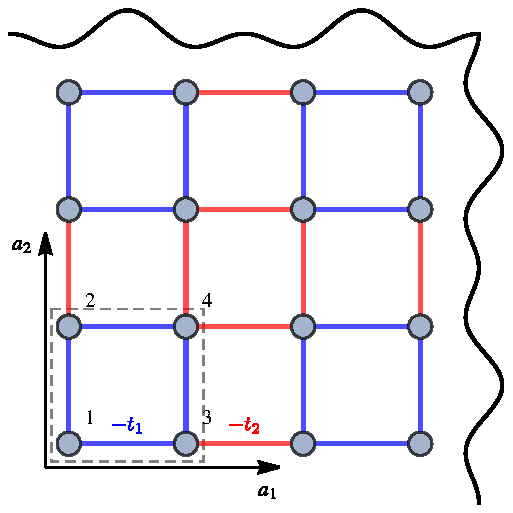
\includegraphics[width=.8\textwidth]{figures/FigLattice.pdf}
    \caption{在正方晶格上的二维SSHBH模型。
    其中一个晶胞被用灰色虚线方框标出,其中四个子晶格被标记为$\eta=1,\dots,4$。
    晶胞内(晶胞间)跃迁强度是$-t_1$ ($-t_2$),被蓝色(红色)标记。
    实空间原初晶格向量$a_{1,2}$用黑色箭头标出。我们定义这些向量的长度为1,作为长度单位。}
    \label{lattice}
\end{figure}
%%%%%%%%%%%%%%%%%%%%%%%%%%%%%%%%%%%%
这个模型哈密顿量可以在实验上很容易实现,例如在二维时,通过把无自旋的玻色子装在一个正方形光晶格,
并且额外再加一个两倍周期的超光晶格,如图\ref{lattice}式。
在$t_1 / t_2$不是很远离1时,我们知道这个系统有一个由$t / U$调控的,
在Mott绝缘态和超流态的量子相变,
这里$t = (t_1 + t_2)/2$ \cite{Fisher1989}。
在$\mu/U$-$t/U$组成的相图的第$p$个耳垂处,
靠近相边界时,只有三个局域态是相关的,
$| p + \sigma \rangle_i$,$\sigma = - 1, 0, 1$。
我们定义三个相互对易的玻色,
$b_{i, \sigma}^{ \dagger} | 0 \rangle = | p + \sigma \rangle_i$,
它们满足一个完整约束,
$\sum_{\sigma=1}^3 b_{i, \sigma}^{ \dagger} b_{i, \sigma} = 1$。
然后原始的玻色子产生算符可以背写成
$a^{ \dagger}_i = \sqrt{p + 1}
b^{ \dagger}_{i, + 1} b_{i, 0} + \sqrt{p} b_{i, 0}^{ \dagger} b_{i, - 1}$。
略去一个不重要的常数项,
在大$p$极限下,
式\eqref{h}变成了一个赝自旋-1的哈密顿量\cite{Altman2002},
\begin{equation}
  \hat{H}_{\text{spin-1}} = \sum_{\langle i, j \rangle} \tilde{t}_{i   j}
  (\hat{S}_i^x \hat{S}_j^x + \hat{S}_i^y \hat{S}_j^y) +  \sum_i \bigg[\frac{1}{2}U
  (\hat{S}_i^z)^2 - \delta \mu \hat{S}_i^z \bigg], \label{heffspin1}
\end{equation}
这里$\langle i, j \rangle$指最近邻两格点。
这里自旋算符被定义为(其中重复的希腊字符下指标需要被求和)$\hat{S}_i^+ = b_{i, \sigma}^{ \dagger} (S^+)_{\sigma \sigma'} b_{i, \sigma'}$,
$\hat{S}_i^- = (\hat{S}_i^+)^{ \dagger}$和$\hat{S}_i^z = b_{i, \sigma}^{ \dagger} (S^z)_{\sigma \sigma'} b_{i, \sigma'}$,
这里$S^z$和$S^+$是在$z$基下的自旋-1矩阵。
$\delta \mu = \mu - (p - 1 / 2)U \approx \mu - pU$是从第$p$个耳垂中间开始测量的化学势。注意其与这个耳垂的尖端在$p \gg 1$时是重合的。
所以所谓的Lorentz不变线在$\mu / U - t / U$相图上就对应于$\delta \mu = 0$,
在这条线上,在低能、长波极限下,其有效哈密顿量有涌现的Lorentz对称性\cite{Sachdev2017}。
自旋交换相互作用是有重整化的跃迁强度给出,$\tilde{t}_{i   j} = pt_{i   j}$,
我们定义$\tilde{t} = pt = p(t_1+t_1)/2$。
原始的$\mathrm{U} (1)$对称性变成了沿$z$方向的$\mathrm{O} (2)$自旋选择对称性,
原始的超流序参量变成$\psi_i = \langle a_i \rangle \approx \sqrt{p / 2} \langle \hat{S}_i^- \rangle$。

利用一个Gutzwiller型的平均场基态ansatz$\left| \text{GS} \right\rangle = \bigotimes_i | \Phi_0 \rangle_i$,其中
\begin{eqnarray}
      | \Phi_0 \rangle_i &=& \cos \frac{1}{2}\theta \ket{0}_i + e^{i (\eta-\phi) / 2} \sin \frac{1}{2}\theta \nonumber\\
      &&  \times \left( \cos \frac{1}{2}\chi \ket{+1}_i + e^{i \phi } \sin \frac{1}{2}\chi \ket{-1}_i   \right),\nonumber
\end{eqnarray}
平均到每个格点到基态能量是
\begin{equation}
  e_0 = \left( \frac{1}{2}U - \delta \mu \cos \chi \right) \sin^2  \frac{1}{2}\theta - \frac{1}{4} z\tilde{t} (1 + \cos \eta \sin  \chi) \sin^2 \theta , \label{mfe}
\end{equation}
其中$z=2d$是配位数。
注意式\eqref{mfe}是独立于参数$\phi$的,
这是由于系统有$\mathrm{O} (2)$对称性。
我们令$\phi=0$,
在超流相,这对应于自旋极化到$x$方向(同样等价于另$\psi_i$是实数)。
在Lorentz不变线上(即令 $\delta \mu = 0$),
通过最小化式\eqref{mfe},基态对应于$(\theta, \eta, \phi, \chi) = (\bar{\theta}, 0, 0, \pi / 2)$,
这里当$U < 4z \tilde{t}$时,$\bar{\theta} = \arccos (U / 4z \tilde{t})$;
而其他情况下$\bar{\theta} = 0$。
通过一个正则变换,
$c_{i, \alpha}^{ \dagger} = b_{i, \sigma}^{ \dagger} T_{\sigma \alpha}$,其中$\alpha = 0, A, P$(后面我们会解释这里的命名缘由),
这里的幺正矩阵$T(\bar\theta)$是
\begin{equation}
   T(\bar\theta) = \begin{bmatrix}
           \frac{1}{\sqrt{2}} \sin \frac{1}{2}\bar{\theta} & \frac{- 1}{\sqrt{2}}     \cos \frac{1}{2}\bar{\theta} & \frac{1}{\sqrt{2}}\\
     \cos \frac{1}{2}\bar{\theta} & \sin \frac{1}{2}\bar{\theta} & 0\\
     \frac{1}{\sqrt{2}} \sin \frac{1}{2}\bar{\theta} & \frac{- 1}{\sqrt{2}}     \cos \frac{1}{2}\bar{\theta} & - \frac{1}{\sqrt{2}}
  \end{bmatrix},\nonumber
\end{equation}
平均场基态是$\left| \text{GS} \right\rangle = \prod_i c_{i,0}^{ \dagger} |0 \rangle$。
为了计算激发谱,
我们凝聚$c_{i,0}^{(\dagger)}$玻色子,
然后把其他模都当作小的扰动。
即我们在式\eqref{heffspin1}中做如下替换$c_{i, 0}^{( \dagger)} \rightarrow \sqrt{1 - \sum_{\alpha \neq 0} c_{i, \alpha}^{ \dagger} c_{i, \alpha}}$ \cite{Auerbach1994},
并且只保留最高到二阶的算符。
这里的零阶给出了平均场基态能量;
一阶项恒等于零;
二阶项可写成两个解耦的哈密顿量,
$\hat{H}^{(2)} = \hat{H}_{A}^{(2)} + \hat{H}_{P}^{(2)}$。
在动量空间,这些哈密顿量可以被写成BdG形式(以下为了简便,我们忽略指标$\alpha$),
$\hat{H}^{(2)} = \frac{1}{2} \sum_{\bm{k}}\chi^{ \dagger}_{\bm{k}} H^{\text{BdG}}_{\bm{k}} \chi_{\bm{k}}$。
这里的Nambu旋量被定义为$\chi_{\bm{k}} = \left[\begin{array}{cc}
c_{\bm{k}} & c_{-\bm{k}}
\end{array}\right]^T$,
其中$c_{\bm{k}}$是一个有$2^d$个分量的算符,
$c_{\bm{k}, \eta}$,
这里$\eta = 1, \ldots, 2^d$是子晶格算符。
这里的BdG矩阵是
\begin{equation}
  H^{\text{BdG}}_{\bm{k}} = \left[\begin{array}{cc}
    gI_{2^d\times 2^d} + \lambda M_{\bm{k}} & \eu^{- \iu \vartheta} \lambda M_{\bm{k}}\\
    \eu^{\iu \vartheta} \lambda M_{\bm{k}} & gI_{2^d\times 2^d} + \lambda M_{\bm{k}}
  \end{array}\right], \label{hbdgspin1}
\end{equation}
这里$M_{\bm{k}}$是$d$维SSH模型的Bloch哈密顿量,
其他参数都在表\ref{tab:parameters}中给出。%
%%%%%%%%%%%%%%%%%%%%%%%%%%%%%%%%%
\begin{table}[htb]
\centering
\caption{被用于式\eqref{hbdgspin1}的参数,分别对于Higgs振幅模($\alpha = A$)和相位模($\alpha = P$)。
注意$\bar\theta=\arccos(U/4z\tilde t)$当$U<4z\tilde t$,反之$\bar\theta =0$。}
\label{tab:parameters}
\begin{tabular}{cccccccc}
\toprule
 &$g$ &$\lambda$ &$\vartheta$\\
\midrule
$\alpha=A$ & $2z\tilde t \sin^2\bar\theta +\frac{1}{2}U\cos\bar\theta$ & $\cos^2\bar\theta$ & $0$ \\
$\alpha=P$ & $z\tilde t\sin^2\bar\theta + \frac{1}{2}U\cos^2\frac{1}{2}\bar\theta$ & $\cos^2\frac{1}{2}\bar\theta$ & $\pi$\\
\bottomrule
\end{tabular}
\end{table}
%%%%%%%%%%%%%%%%%%%%%%%%%%%%%%%%%
对角式\eqref{hbdgspin1}的Bogoliubov变换可以解析地从无相互作用哈密顿量$M_{\bm{k}}$得到 \cite{Kumar2020}。
具体来说,
假设幺正矩阵$Q_{\bm{k}}$对角$M_{\bm{k}}$,
$Q_{\bm{k}}^{ \dagger} M_{\bm{k}} Q_{\bm{k}} = \text{diag} \{m_{1, \bm{k}}, \ldots, m_{2^d, \bm{k}} \}$,
我们定义两个双曲线函数$\cosh\beta_{i, \bm{k}} = \sqrt{\frac{g + m_{i, \bm{k}}}{2 E_{i,\bm{k}}} + \frac{1}{2}}$和
$\sinh \beta_{i, \bm{k}} = - \sgn(m_{i, \bm{k}}) \sqrt{\frac{g_{\alpha} + m_{i, \bm{k}}}{2 E_{i,\bm{k}}} - \frac{1}{2}}$,
其中
\begin{equation}
  E_{i, \bm{k}} = \sqrt{g^2 + 2 g m_{i, \bm{k}}}, \label{eb}
\end{equation}
我们还定义两个相关的对角矩阵$C_{\bm{k}} = \text{diag} \{ \cosh \beta_{1, \bm{k}}, \ldots, \cosh \beta_{2^d,\bm{k}} \}$,
和$S_{\alpha, \bm{k}} = \text{diag} \{ \sinh \beta_{1,\bm{k}}, \ldots, \sinh \beta_{2^d, \bm{k}} \}$。
那么这里被需要的赝幺正变换是
\begin{equation}
  W_{\bm{k}}^{ \dagger} (\Sigma_z H^\bdg_{\vb k}) W_{\bm{k}}  = \tau_z \otimes \begin{bmatrix}
      E_{1, \bm{k}} & & \\
      & \ddots & \\
      & & E_{2^d,\bm{k}}
  \end{bmatrix},\label{put}
\end{equation}
其中$\Sigma_z=\tau_z\otimes I_{2^d}$。
这里的赝幺正矩阵是$W_{\bm{k}} = \tilde Q_{\bm{k}} P_{\bm{k}}$,
其中$\tilde Q_{\bm{k}}=\tau_0 \otimes Q_{\bm{k}}$,
和$P_{\bm{k}} = \tau_0 \otimes C_{\bm{k}} + \tau_1 \otimes S_{\bm{k}}$,
而$\tau_i$,$i=1,2,3$和$i=0$,
分别是三个Pauli矩阵,和$2\times 2$单位矩阵,
作用在Nambu空间。

%%%%%%%%%%%%%%%%%%%%%%%%%%%%%%%%%%%%%%%
\begin{figure}[t]
\centering
    \includegraphics[width=.9\textwidth]{FigSpin1OBC.pdf}
    \caption{二维SSHBH模型在一个带状几何上的激发谱。
    (a) ($t_1/t_2=3$) 和 (b) ($t_2/t_1=3$) 对应于Higgs振幅模。
    (c) ($t_1/t_2=3$) 和 (d) ($t_2/t_1=3$) 对应于相位模。
    分别是两重简并的(由于空间反演对称性)两条蓝线,对应于拓扑边界态,它们的波函数有超过$66\%$ 的比例局域在边界的晶胞上。
    其他参数:
    $U=0.95 U_c$,其中$U_c=4z \tilde t$对应于相变点。}
    \label{spin1OBC}
\end{figure}
%%%%%%%%%%%%%%%%%%%%%%%%%%%%%%%%%%%%%%%

对于一个由动量$\bm{k}$和能带指标$\lambda$标记的低能激发,它会对给定一个算符$O_i$的基态平均值产生扰动,$\delta O_i = \expval{O_i}_{\bm k,\lambda}-\expval{O_i}_0$。
对于自旋算符$\hat{\bm{S}}_i$,
最高到微扰的线形阶,
由于两种模$\alpha = A$和$P$导致的这种振荡是
\begin{subequations}\label{per}
    \begin{align}
        \delta \bm{S}_i^{(A)} &= f^{(A)}_{\bm{k}, \lambda} \cos (E_{i, \alpha,
  \bm{k}} t -\bm{k} \cdot \bm{r}) \hat{\bm{e}}_x,
  \label{dsa}\\
   \delta \bm{S}_i^{(P)} &= f^{(P)}_{ \bm{k}, \lambda} \sin (E_{k,
  \lambda} t -\bm{k} \cdot \bm{r}_i) \hat{\bm{e}}_y \nonumber\\
 &\quad + f^{(P)\prime}_{\bm{k}, \lambda} \cos (E_{k, \lambda} t -\bm{k} \cdot
  \bm{r}_i) \hat{\bm{e}}_z, \label{dsp}
    \end{align}
\end{subequations}
这里的三个系数是$f^{(A)}_{\bm{k}, \lambda} = - [Q_{\bm{k}}]_{\eta \lambda} g^{(A)}_{\lambda, \bm{k}} \cos \bar{\theta}$,
$f^{(P)}_{\bm{k}, \lambda}= - [Q_{\bm{k}}]_{\eta \lambda} g^{(P)}_{\lambda, \bm{k}} \cos\frac{1}{2}\bar{\theta}$和$f^{(P)\prime}_{\bm{k}, \lambda} = -[Q_{\bm{k}}]_{\eta \lambda} g^{(P)}_{\lambda, \bm{k}} \sin\frac{1}{2}\bar{\theta}$,
其中$g^{(\alpha)}_{\lambda, \bm{k}} = \sinh\beta^{(\alpha)}_{\lambda, \bm{k}} + \cosh \beta^{(\alpha)}_{\lambda,
\bm{k}}$。通过合适选取矩阵$Q_{\bm{k}}$的规范,上述系数可以全部变成实数。
式\eqref{dsa}因此确认了$A$模是Higgs振幅模,因为它们导致了自旋的集体纵向振荡;类似地,式\eqref{dsp}确认了$P$模是相位模(即磁子),因为它们导致了自旋的集体横向振荡(即进动)。
额外地,注意到
\begin{equation}
  \delta\psi_i = (\rho_0 + \delta \rho_i) \eu^{\iu \delta \phi_i} - \rho_0
  \approx \delta \rho_i + \iu \rho_0 \delta \phi_i, \label{op}
\end{equation}
所以完全的振幅$\rho$和相位$\phi$振荡分别对应于$\delta \psi_i$没有虚部和实部。
由于$a_i \propto S_i^- = S_i^x - \iu S_i^y$,这等价于自旋没有在$y$和$x$方向的扰动。
所以用原始玻色子的语言,式\eqref{per}同样确认了完全的Higgs振幅模在大$p$极限下是存在的。

现在我们证明Higgs振幅模的拓扑性质直接继承于$d$维的SSH模型。
回忆后者是一个由空间反演对称性保护的拓扑晶体绝缘体,
\begin{equation}
  \mathcal{I}M_{\bm{k}} \mathcal{I}^{- 1}  =M_{-\bm{k}}, \label{is0}
\end{equation}
其对应的拓扑不变量是向量化的Zak相,同时也等于宏观极化矢量,被定义为\cite{Liu2017}
\begin{equation}
  \bm{P}= \frac{1}{2 \pi} \int \dif^2 k \Tr [\bm{A}
  (\bm{k})], \label{mpv}
\end{equation}
这里的Berry联络是$A_i = \iu \sum_{\lambda\leq\lambda_{\text{max}}} \Tr [\Gamma_\lambda Q^{ \dagger}_{\bm{k}} \partial_{k_i} Q_{\bm{k}}]$,$i=x_1,\dots,x_d$,其中$\Gamma_\lambda$是一个$2^d\times 2^d$矩阵,只有第$\lambda$个对角元素是$+ 1$,其他所有都为零。
$\lambda_{\text{max}}$是所有被占据能带中最大的那个能带指标。
积分区间是整个布里渊区。
由于空间反演对称性,
$\bm{P}$的每个分量都是严格量子化到一个$\mathbb{Z}_2$数到\cite{Fang2012},
\begin{equation}
  P_i = \frac{i}{2 \pi} \ln \left[ \prod_{\lambda\leq\lambda_{\text{max}}} \eta_{\lambda} (\Gamma)
  \eta_{\lambda} (X_i) \right], \label{p}
\end{equation}
这里$\eta_{\lambda}$是空间反演算符$\mathcal I$的对于第$\lambda$个能带的本征值,$X_i$是第一布里渊区在$x_i$上不同于$\Gamma$的空间反演对称不变动量。
能带翻转点同时发生在所有$X_i$处,当$t_1 = t_2$时,这是因为,例如在二维时,$\mathrm{C}_{4v}$对称性。
对于$t_1 < t_2$,
系统处在拓扑相,
这时$\bm{P}= \left(1/2,\dots, 1/2 \right)$;
反之,则系统处在平凡相,有$\bm{P}= (0,\dots, 0)$。
回到定义在式\eqref{hbdgspin1}的玻色型BdG系统,
这里的我们需要将单粒子的空间反演对称算符提升到包含Nambu空间的算符$\mathcal{I}_{\tau} = \tau_0 \otimes \mathcal{I}$,
这时空间反演对称性被定义为
\begin{equation}
  \mathcal{I}_{\tau} H^{\text{BdG}}_{\bm{k}} \mathcal{I}_{\tau}^{- 1} = H^{\text{BdG}}_{-\bm{k}},\label{is}
\end{equation}
其对应的拓扑不变量同样由式\eqref{mpv}给出,
这里玻色型Berry联络是$A_i = \iu \sum_{\lambda\leq\lambda_{\text{max}}} \Tr [\Gamma_\lambda \Sigma_3 W_{\bm{k}}^{ \dagger} \Sigma_3 \partial_{k_i} W_{\bm{k}}]$ \cite{Shindou2013}。
这样定义的$\bm{P}$被称为向量化的辛极化,
它同样由于空间反演对称性而被量子化\cite{Engelhardt2015},
同样被式\eqref{p}给出。
利用定义在式\eqref{put}中的$W_{\bm{k}}$,
容易得到
\begin{equation}
  W_{\bm{K}}^{ \dagger} \Sigma_z \mathcal{I}_\tau W_{\bm{K}} = \tau_z
  \otimes \begin{bmatrix}
      \eta_{1,\bm{K}} & &\\
      & \ddots & \\
      & & \eta_{2^d,\bm{K}}
  \end{bmatrix} ,\nonumber
\end{equation}
这里$\bm{K}$是一个空间反演对称动量。
所以BdG系统的空间反演算符本征值与对应的$d$维SSH模型完全一样。
而且式\eqref{eb}暗示了BdG系统的能谱也是一个关于对应的$d$维SSH模型能谱的光滑、单调递增函数。
所以对于这个BdG系统,它的拓扑($t_1 < t_2$)和平庸($t_1 > t_2$)激发谱转变点也是发生在$t_1 = t_2$。

根据体边对应,一个非平庸的体拓扑数暗示了当取开放边界条件时,拓扑边界态的存在。对于Higgs振幅能带和相位能带,通过选取一个带状几何,我们数值地确认了体边对应的确成立,如图\ref{spin1OBC}所示。

%%%%%%%%%%%%%%%%%%%%%%%%%%%%%%%%%%%%%%%
\begin{figure*}
\centering
    \includegraphics[width=\textwidth]{FigSBPBCOBC.pdf}
    \caption{二维SSHBH模型在(a)周期性边界条件下(b)开放边界条件下的激发谱,其中颜色暗示了对于激发的平坦度,定义在式\eqref{flatness}。
    这里的填充数$p=2$,对于 (a1)、(b1);
    $p=30$,对于(a2)、(b2);
    $p=120$,对于(a3)、(b3)。
    (b)图中那些更大的点对应于拓扑边界态。其他参数:$U=0.95 U_c$, $t_2/t_1=3$,化学势$\mu$的选取是使系统在Lorentz不变线上。}
    \label{pbcobc}
\end{figure*}
%%%%%%%%%%%%%%%%%%%%%%%%%%%%%%%%%%%%%%%

\section{拓扑Higgs振幅模在有限填充下的命运}

虽然我们已经证实了拓扑的Higgs模在大填充数极限下是存在的,但是实验上更相关的是考察有限填充数时这些模式的命运,即它们是否还存在。
用赝自旋-1的语言,有限填充的情况等价于引入了一些最近邻的三或者四自旋点相互作用项 \cite{Huber2007},这让讨论变得笨拙而且没有必要。
这里我们利用一个slave boson (SB)方法\cite{Frerot2016}直接处理式\eqref{h},
从一个强耦合平均场出发。
即,我们先自洽地解一系列平均场哈密顿量,
\begin{equation}
  \hat{H}_i^{\tmf} = \sum_j (a_i^{\dag} t_{i   j} \phi_j +
   \mathrm{h.c.}) - \mu a_i^{\dag} a_i +
   \frac{1}{2}U a^{\dag}_i a_i^{\dag} a_i a_i,\nonumber
\end{equation}
这里$\phi_i = \langle \Phi_{i 0} | a_i | \Phi_{i 0} \rangle$是基态期望值。
这个解提供了局域的本征基$\{ | \Phi_{i \alpha} \rangle, \alpha = 0, 1, \ldots, n_c \}$,
其中本征能量$\varepsilon_{i \alpha}$按升序排列,$n_c$是局域Hilbert空间维度的截断。
SB算符$b_{i \alpha}$被定义为$a_i = \sum_{\alpha, \beta \geqslant 0} \mathcal{A}_{i, \alpha \beta} b_{i \alpha}^{\dag} b_{i \beta}$,
其中$\mathcal{A}_{i, \alpha \beta} = \langle \Phi_{i \alpha} | a_i | \Phi_{i \beta} \rangle$,$\mathcal{A}_{i, \alpha \beta}^{\dag} = \langle \Phi_{i\alpha} | a_i^{\dag} | \Phi_{i \beta} \rangle$。
它们满足一个局域限制条件,$\sum_{\alpha \geqslant 0} b_{i \alpha}^{\dag} b_{i \alpha} = 1$,
这保证了上述映射是正则的\cite{Huerga2013}。
式\eqref{h}可以用SB算符严格地重写为
\[ \hat{H} = \sum_{i   j} \sum_{\alpha \beta \gamma \theta} b_{i
   \alpha}^{\dag} b_{i \beta} F_{i \alpha \beta, j \gamma \sigma} b_{j
   \gamma}^{\dag} b_{j \sigma} + \sum_i \sum_{\alpha \beta} b_{i
   \alpha}^{\dag} G_{i, \alpha \beta} b_{i \beta}, \]
这里$F_{i \alpha \beta, j \gamma \sigma} =\mathcal{A}_{i, \alpha \beta}^{\dag} t_{i   j} \mathcal{A}_{j, \gamma \sigma}$,$G_{i, \alpha \beta} = \left\langle \Phi_{i,\alpha} \left| \left[ \frac{1}{2}U (\hat{n}_i - 1) \hat{n}_i - \mu \hat{n}_i \right] \right| \Phi_{i, \beta} \right\rangle$。
为了算低能激发,我们通过凝聚$b_{i 0}$ (即,取近似$b_{i,0}^{(\dagger)}\rightarrow \sqrt{1-\sum_{\alpha> 0} b_{i \alpha}^{\dag} b_{i \alpha}}$)来得到一个二次型的扰动哈密顿量,
\begin{eqnarray}
      \hat{H}^{(2)} &=& \sum_{\alpha, \beta > 0} \bigg[ \sum_{i   j} b_{i
  \alpha}^{\dag} A_{i \alpha, j \beta} b_{j \beta}\nonumber\\
  && + \frac{1}{2} \left(
  \sum_{i   j} b_{i \alpha}^{\dag} B_{i \alpha, j \beta} b_{j
  \beta}^{\dag} + \text{H.c.} \right) \bigg],\nonumber
\end{eqnarray}
这里$A_{i \alpha, j \beta} = \delta_{i   j} \delta_{\alpha \beta} (\varepsilon_{i \alpha} - \varepsilon_{i 0}) + F_{i \alpha 0, j 0 \beta} + F_{j 0 \beta, i \alpha 0}$,$B_{i \alpha, j \beta} = F_{i \alpha 0, j \beta 0} + F_{j \beta 0, i \alpha 0}$。
在动量空间,我们定义Nambu旋量$\beta_{\bm{k}} =
\left[\begin{array}{cc}
  b_{\bm{k}} & b_{-\bm{k}}^{\dag}
\end{array}\right]^T$,
其中$b_{\bm{k}}$是一个有$n_c \times 2^d$个分量的算符$b_{\bm{k} \alpha \eta}$,这里$\alpha = 1, \ldots, n_c$,$\eta = 1, \ldots, 2^d$标记子晶格。
其对应的BdG方程是
\[ H^{\text{BdG}}_{\bm{k}} = \left[\begin{array}{cc}
     A_{\bm{k}} & B_{\bm{k}}\\
     B_{-\bm{k}}^{\ast} & A_{-\bm{k}}^T
   \end{array}\right], \]
   其中$[A_{\bm{k}}]_{\eta\alpha,\eta'\beta} = \sum_{\bm{r}_l -\bm{r}_{l'}} \eu^{-\iu \bm{k} \cdot (\bm{r}_l -\bm{r}_{l'})} A_{l \eta\alpha, l' \eta' \beta}$,
   $[B_{\bm{k}}]_{\eta\alpha,\eta'\beta} = \sum_{\bm{r}_l-\bm{r}_{l'}} \eu^{- \iu \bm{k} \cdot (\bm{r}_l-\bm{r}_{l'})} B_{l \eta \alpha, l' \eta' \beta}$,
   $\bm{r}_l$和$\bm{r}_{l'}$是元胞坐标。
   由于局域基也满足空间反演对称性,$\ket{\Psi_{i\alpha}}=\ket{\Psi_{\bar i\alpha}}$,
   其中两个格点坐标是通过反演对称操作联系的$\hat{\mathcal I}: i\rightarrow\bar i$。
   所以这个BdG哈密顿量仍然满足一个如式\eqref{is}的空间反演对称性,
   不过这里的空间反演对称算符变成了$\tau_0\otimes I_{2^d}\otimes \mathcal I$。
   对应的体拓扑不变量仍由式\eqref{p}给出。
   而且由于(例如在二维时)$\mathrm{C}_{4v}$对称性,能带翻转点仍同时发生在所有$X_i$处,
   并且仍发生在$t_1=t_2$时,后者可以启发式地解释为由于$t_1$和$t_2$扮演者对称的角色。所以激发谱的拓扑结构在有限填充时仍然存在,而且其拓扑-平庸转变边界也没有发生变化。
   
   接下来我们关注这些激发谱的振幅-相位特征。
   通过一个Bogoliubov变换$\chi_{\bm{k}} = T_{\bm{k}} \beta_{\bm{k}}$,其中
\begin{equation}
  T_{\bm{k}} = \left[\begin{array}{cc}
  U_{\bm{k}} & - V_{\bm{k}}\\
  - V_{-\bm{k}}^{\ast} & U_{-\bm{k}}^{\ast}
\end{array}\right],\ T_{\bm{k}}^{- 1} = \Sigma_3
T_{\bm{k}}^{\dag} \Sigma_3 = \left[\begin{array}{cc}
  U_{\bm{k}}^{\dag} & V_{-\bm{k}}^T\\
  V_{\bm{k}}^{\dag} & U_{-\bm{k}}^T
\end{array}\right].\nonumber
\end{equation}
我们可以得到激发谱$\omega_{\bm{k} \lambda}$,$\lambda = 1, \ldots, 2^d\times n_c$,它们以升序排列。序参量$\psi_i=\langle a_i \rangle$由于一个由动量$\bm{k}$和能带指标$\lambda$标记的激发导致的扰动是
\[ \delta \psi_\eta = X_{\eta, \bm{k}\lambda} e^{- i
   (\omega_{\bm{k}\lambda} t -\bm{k} \cdot \bm{r}_i)} + Y_{\eta,
   \bm{k}\lambda} e^{i (\omega_{\bm{k}\lambda} t -\bm{k} \cdot
   \bm{r}_i)}, \]
其中
\begin{eqnarray*}
  X_{\eta, \bm{k}\lambda} & = & \sum_{\alpha > 0} [\mathcal{A}_{\eta, \alpha
  0} (V_{\bm{k}}^{\dag})_{\alpha \lambda} +\mathcal{A}_{\eta, 0 \alpha}
  (U^{\dag}_{\bm{k}})_{\alpha \lambda}],\\
  Y_{\eta, \bm{k}\lambda} & = & \sum_{\alpha > 0} [\mathcal{A}_{\eta, \alpha
  0} (U^T_{\bm{k}})_{\alpha \lambda} +\mathcal{A}_{\eta, 0 \alpha}
  (V_{\bm{k}}^T)_{\alpha \lambda}] .
\end{eqnarray*}
正如式\eqref{op}所示,
序参量完整的振幅(相位)振荡对应于$\delta \psi_i$的虚部(实部)为零,即
$I_{\bm{k}\lambda} = X_{\bm{k}\lambda} - Y_{\bm{k}\lambda} = 0$ ($R_{\bm{k}\lambda} = X_{\bm{k}\lambda} + Y_{\bm{k}\lambda} = 0$)。
我们定义一个平坦度 \cite{Liberto2018}
\begin{equation}
  F_{\bm{k}\lambda} = \frac{| R_{\bm{k}\lambda} | - | I_{\bm{k}\lambda} |}{|
   R_{\bm{k}\lambda} | + | I_{\bm{k}\lambda} |} \in [- 1, 1],\label{flatness}
\end{equation}
来量化一个振荡的振幅和相位分量:一个正的(负的)平坦度意味着支配的振幅(相位)特征。
一个完全的振幅(相位)振荡对应于$F_{\bm{k}\lambda} \rightarrow 1$ ($- 1$),
而这个条件显然也被大填充极限下的$A$ ($P$)模满足。
在图\ref{pbcobc}中,
我们展示了在取周期性边界条件和开放边界条件时的激发谱,
同时用颜色标记了每个模对应的平坦度。
从图中我们可以看出随着填充数降低,越来越多的态会失去它们的振幅/相位特性,从高能量态开始。
但是在一个比较合理、实验允许的填充$n_0=120$,
拓扑的Higgs振幅边界态已经衍生出来、可以被实验测量了。


%%%%%%%%%%%%%%%%%%%%%%%%%%%%%%%%%%%%%%%%%%%%%%%%%%%%%%%%%%%%%%%%%%%%%%
\section{来自Ginzberg-Landau分析的洞察}

最后我们给出一个互补、简单、统一的图像来解释以上结果。
注意到在一个整数填充$p\in \mathbb Z_{\geq 0}$,
靠近SF-MI相变点时,我们可以用一个强耦合RPA方法\cite{Sengupta2005}得到这个$d$维SSHBH模型的低能有效作用量,
\begin{eqnarray}
      S_{\text{eff}} &=& \int \dif \tau \sum_{i  } \psi_i^{\ast} \left[
  \sum_{l = 0}^{\infty} (- 1)^{l + 1} c_l \partial^l_{\tau} \right] \psi_i\nonumber\\
  && +
  \sum_{i   j} \psi_i^{\ast} t_{i   j} \psi_j +
  \frac{\tilde{U}}{2} \sum_i \psi_i^{\ast} \psi_i^{\ast} \psi_i \psi_i,\nonumber
\end{eqnarray}
其中$c_l = \frac{1}{l!} \frac{\partial^l G^{- 1}_{\text{loc}} (\iu
\omega)}{\partial (\iu \omega)^l} |_{\iu \omega = 0}$,$l=0,1,\dots$,$G_{\text{loc}} (\iu \omega_n) = \frac{- p}{i\omega_n + \varepsilon_{p - 1} - \varepsilon_p} + \frac{p + 1}{i \omega_n +
\varepsilon_p - \varepsilon_{p + 1}}$是严格的零温局域传播子,
$\varepsilon_p = - \mu p + (U / 2) p (p - 1)$是在局域极限下的本征能量。
注意到上式中裸的相互作用强度$U$已经被换成了严格的局域两粒子顶点函数,在静态极限下。它是一个关于$p$, $\mu$和$U$的函数,但其一般形式跟我们以下讨论无关。
在超流相,利用一个格点无关的序参量$\psi_i = \psi_0 \in \mathbb{R}$,
并且引入如式\eqref{op}那样的扰动,一个二次型扰动作用量可以被得到\footnote{
注意跃迁项没有非对角元贡献跟无相互作用哈密顿量的具体形式相关。容易证明对于一个无自旋玻色子,如果凝聚体波函数是格点无关的,那么一个复数形式的跃迁系数总是导致相位和振幅模的耦合。}
\begin{align}
  S^{(2)} &= \int \dif \tau \sum_{i   j} \left[\begin{array}{cc}
     \rho_i & \theta_i
   \end{array}\right]  \nonumber\\
  &\quad \times \left[\begin{array}{cc}
    t_{ij}- \sum_{n = 0}^{\infty} c_{2 n} \partial_{\tau}^{2 n} - \tilde{\mu} + 3
    \tilde{U} \psi_0^2 & \iu \psi_0 \delta_{i   j} \sum_{n =
    0}^{\infty} c_{2 n + 1} \partial_{\tau}^{2 n + 1}\\
    - \iu \psi_0 \delta_{i   j} \sum_{n = 0}^{\infty} c_{2 n + 1}
    \partial_{\tau}^{2 n + 1} & t_{ij}+\psi_0^2 \left( - \sum_{n = 0}^{\infty} c_{2
    n} \partial_{\tau}^{2 n} - \tilde{\mu} + \tilde{U} \psi_0^2 \right)
  \end{array}\right] \left[\begin{array}{c}
     \rho_j\\
     \theta_j
   \end{array}\right]. \label{hij}
\end{align}    
通过令$c_1 = 0$ (即,在Lorentz不变线上),并且在低能极限下$\omega \rightarrow 0$,
式\eqref{hij}中的所有非对角贡献都是零,
所以通常定义的Higgs振幅模是良好定义的。
这解释了为什么在图\ref{pbcobc}中,对于任意填充数,完全的Higgs振幅/相位模在低能极限下会持续存在。
注意到在Lorentz不变线上,
容易证明$c_l |_{\text{LIL}} =\mathcal{O} (p^{- l+ 1})$,对于$l \geq 2$。
所以在大$p$极限下,相对于其他$c_l$,$l>2$,只有$c_2$能留下来,所以这时非对角元也等于零。
此外,
由于跃迁项并没有发生改变,这两种解耦的模直接继承了$d$维SSH模型的拓扑。
最后,在有限填充情况下,即使在Lorentz不变线上,非对角元仍有耦合,其强度由$1/p$压制,并且是在位的、满足空间反演对称性的。所以激发谱的拓扑性质在有限填充下仍然存在,但是高能量态的振幅-相位特征逐渐消失。

\section{小结和讨论}

用$d$维的SSHBH模型作为例子,我们证实了在量子相变临界点附近拓扑的Higgs振幅模存在。具体地,我们展示了在大填充数极限下衍生的拓扑Higgs振幅能带和相位能带,它们的拓扑性质直接继承于$d$维的SSH模型,即体拓扑不变量是一个$\mathbb Z_2$数,被称为向量化的辛极化,其量子化的性质是由空间反演对称性保护的。我们还数值证明了体边对应关系。
当减小填充数时,激发谱的拓扑性质没有变化,但是高能量态的振幅-相位特性逐渐消失。我们利用定义的一个平坦度来量化了这些激发态的振幅/相位振荡特征,并且数值地展示了,在实验可实现的范围内,当填充数取到足够大,拓扑边界态变成支配的Higgs振幅模特征。最后,利用强耦合RPA方法,我们分析了得到低能有效作用量,互补、统一地解释了前述结果。

有一些直接的问题留给未来继续研究。这里讨论的拓扑Higgs振幅模只在经典(二次型)层面是长寿命的,它们是否能在考虑量子修正时仍然存活?它们是否是过阻尼的 \cite{Podolsky2011}?
另外,一个有意思的推广是,类似的拓扑Higgs振幅模是否在其他凝聚态体系存在:例如当拓扑超导体或者拓扑量子磁性体系处在量子临界点附近时。
